%%%%%%%%%%%%%%%%%%%%%%%%%%%%%%%%%%%%%%%%%%%%%%%%%%%%%%%%%%%%%%%%%%%%%%%%%%%%%%%%
\newcommand{\framerowsynth}[1]{%
\adjustbox{valign=m,vspace=1pt}{\includegraphics[width=2.25cm,height=2.5cm]{face_flow/images/synthetic/#1_gt}}                &
\adjustbox{valign=m,vspace=1pt}{\includegraphics[width=2.25cm,height=2.5cm]{face_flow/images/synthetic/#1_ff_dsift_sequence}} &
\adjustbox{valign=m,vspace=1pt}{\includegraphics[width=2.25cm,height=2.5cm]{face_flow/images/synthetic/#1_ff_dsift_single}}   &
\adjustbox{valign=m,vspace=1pt}{\includegraphics[width=2.25cm,height=2.5cm]{face_flow/images/synthetic/#1_mfsf}}              &
\adjustbox{valign=m,vspace=1pt}{\includegraphics[width=2.25cm,height=2.5cm]{face_flow/images/synthetic/#1_ldof}}              &
\adjustbox{valign=m,vspace=1pt}{\includegraphics[width=2.25cm,height=2.5cm]{face_flow/images/synthetic/#1_epicflow}}          &
\adjustbox{valign=m,vspace=1pt}{\includegraphics[width=2.25cm,height=2.5cm]{face_flow/images/synthetic/#1_siftflow}}
}
\setlength{\tabcolsep}{1pt}
\begin{figure}[t]
    \centering
    \begin{tabular}{cccccccc}
        & GT & FF LR & FF FR & MFSF & LDOF & EPICFlow & SIFTFlow \\ \vspace{-0.3cm}
        16 & \framerowsynth{16}                                  \\ \vspace{-0.3cm}
        54 & \framerowsynth{54}                                  \\ \vspace{-0.3cm}
        139 & \framerowsynth{139}                                \\
        233 & \framerowsynth{233}
    \end{tabular}
    \caption{Example endpoint results for the synthetic sequence including
             illumination variation. Each row shows a different frame of the
             280 frame synthetic sequence (Frame 16, 54, 139 and 233 from top
             to bottom)}
\label{fig:synthetic_examples}
\end{figure}
\setlength{\tabcolsep}{6pt}
%%%%%%%%%%%%%%%%%%%%%%%%%%%%%%%%%%%%%%%%%%%%%%%%%%%%%%%%%%%%%%%%%%%%%%%%%%%%%%%%
%%%%%%%%%%%%%%%%%%%%%%%%%%%%%%%%%%%%%%%%%%%%%%%%%%%%%%%%%%%%%%%%%%%%%%%%%%%%%%%%
\section{Experiments}\label{sec:experiments}
%%%%%%%%%%%%%%%%%%%%%%%%%%%%%%%%%%%%%%%%%%%%%%%%%%%%%%%%%%%%%%%%%%%%%%%%%%%%%%%%
In this section, we describe the set of qualitative and quantitative experiments
that we conducted in order to demonstrate the effectiveness of our proposed algorithm,
Face Flow. In order to verify that our method is competitive with the state-of-the-art,
we compared against the methods of
\citet{Garg:2013hu} (denoted MFSF),
\citet{revaud2015epicflow} (denoted EPICFlow),
\citet{Liu:2011jv} (denoted SIFTFlow) and the large displacement
optical method of \citet{Brox:2011be} (denoted LDOF). We also provide two
formulations of our method, one which enforces the low-rank constraint on the coefficients
and one which does not. The latter corresponds to the choice of $\lambda=k$.
We denote these two methods Face Flow Low-Rank (LR) and Face Flow
Full-Rank (FR). This self evaluation is particularly useful for demonstrating the importance
and effectiveness of the low-rank constraint for multi-frame facial flow.

To effectively evaluate Face Flow, we propose a novel ground truth dataset formed
from facial motion capture data~\cite{zhang2008spacetime}. The sequence that we
evaluate must be in correspondence and ideally contain an interesting
sequence of deformations. Performance capture data is ideal for this purpose, as
it is necessarily in correspondence and often deals with actors portraying
scripted, emotional content. We also evaluate face flow on a realistic sequence
portraying a number of common issues in facial videos, including motion blur
and occlusions. Please see the supplementary material for
video examples of the sequences and further results.
%%%%%%%%%%%%%%%%%%%%%%%%%%%%%%%%%%%%%%%%%%%%%%%%%%%%%%%%%%%%%%%%%%%%%%%%%%%%%%%%
\subsection{Practical Deformation Basis Construction}\label{subsec:experiments_basis}
%%%%%%%%%%%%%%%%%%%%%%%%%%%%%%%%%%%%%%%%%%%%%%%%%%%%%%%%%%%%%%%%%%%%%%%%%%%%%%%%
Our facial deformation basis is built by applying MFSF multi-frame optical flow method
\footnote{Code publicly available at https://bitbucket.org/troussos/mfsf/} of \citet{Garg:2013hu} on
the facial expression database BU4D~\cite{bu4d}. We chose this database due
to the large range of expression present and the fact that is captured at a high
frame rate, which is ideal for the technique of \citet{Garg:2013hu}. However, in order
to further improve the performance of \citet{Garg:2013hu}, we augmented the energy
to include an extra quadratic landmark constraint. This landmark constraint
takes a similar form to the landmark constraint proposed in this paper, and was
found to improve the results considerably in sequences that displayed particularly
expressive emotion, such as surprise.

The BU4D database consists of 102 subjects displaying 6 canonical expression,
from neutral to the apex of the emotion. We selected a neutral frame for every
sequence and used this as the reference frame for the method of \citet{Garg:2013hu}.
After computing trajectories for each sequence,
we constructed a reference frame for our deformation basis using the mean
of the neutral images we selected previously. We then applied principal
component analysis (PCA) to learn the linear deformation model as described in Section~\ref{subsec:learning_deformation}.
Experimentally, we found that $k=20$ principal components of
non-rigid deformation accounts for $~95\%$ of the variance.
We note that the BU4D-FE data shows frontal faces and thus our model does not capture out-of-plane
rotation. However, there is no practical reason that our PCA basis could not capture
this kind of deformation.

In order to improve the robustness of our algorithm, we adopt a pseudo coarse-to-fine
strategy for basis construction and create three bases of increasing scale. This is also
commonly employed within optical algorithms to improve robustness. In all of the following experiments,
the feature descriptor employed is the dense SIFT feature.
%%%%%%%%%%%%%%%%%%%%%%%%%%%%%%%%%%%%%%%%%%%%%%%%%%%%%%%%%%%%%%%%%%%%%%%%%%%%%%%%
\subsection{Motion Capture Data}\label{subsec:experiments_mocap}
%%%%%%%%%%%%%%%%%%%%%%%%%%%%%%%%%%%%%%%%%%%%%%%%%%%%%%%%%%%%%%%%%%%%%%%%%%%%%%%%
In this experiment, we use the performance capture dataset provided by \citet{zhang2008spacetime}
to generate three novel ground truth sequences consisting of 280 frames. This ground truth is provided by rendering
the sequence of meshes in a fixed pose, which yields both a texture and a set of vertices
in the scene. These vertices can then be used in order simply calculate flow for the face
throughout the image.

As mentioned, we rendered three sets of texture, all with the same underlying geometry,
to provide evidence of the robustness of Face Flow to challenging conditions. In the first
sequence, we rendered unmodified textures. This is a baseline
in order to show the performance of state-of-the-art methods for facial data. Since
our basis is trained using the output from~\cite{Garg:2013hu}, we do not expect to
outperform other optical flow techniques on this sequence. The second sequence
was rendered by rendering a periodically moving light source around the face. This
is challenging for the data term and helps to demonstrate the
robustness of our chosen feature descriptor. The final sequence is highly challenging. It contains
the periodic illumination variation from the previous sequence and also an artificial
occlusion in the form of a smoothly translating hand.

In order to initialise our Face Flow algorithm, we manually annotated the first frame
as the reference frame. To obtain an initial estimate of the coefficient
matrix $\mathbf{C}$, the landmark constraint quadratic term is solved, which
provides a reasonable estimate of the initial shape. Once solved in the reference frame,
this initialisation was propagated across every frame in the sequence. The landmark constraint
was otherwise not utilised in this experiment.

To evaluate the performance of the methods, we computed the root mean squared
error of the endpoints (RMSE), shown in Table~\ref{tbl:synthetic}. As expected
Face Flow does not outperform state-of-the-art methods in the original un-tampered
sequence. However, in the more interesting case of the illumination variation
and occlusion sequences, our Face Flow method with low-rank constraint (Face Flow LR),
performs the best. We also note that the low-rank method of our technique significantly
outperforms the full-rank version, particularly in the occluded sequence. An example
set of endpoints is given in Figure~\ref{fig:synthetic_examples}. Note how
the face deformation is well localised and unlikely to undergo any gross deformations
due to being constrained by a statistical basis.

Finally, to provide evidence as to the stability of our algorithm, and the the effect
of the low-rank constraint on the outcome of the sequence, we present Figure~\ref{fig:per_frame_error}.
This figure shows the mean per-frame endpoint error across the sequence. The Face Flow
methods are given by the blue and green lines. Note how stable the Face Flow LR method is,
particularly when compared to the Face Flow FR method. We believe this effectively
demonstrates the positive effect enforcing soft temporal consistency can have.
%%%%%%%%%%%%%%%%%%%%%%%%%%%%%%%%%%%%%%%%%%%%%%%%%%%%%%%%%%%%%%%%%%%%%%%%%%%%%%%%
\subsection{Real Sequence}\label{subsec:experiments_real}
%%%%%%%%%%%%%%%%%%%%%%%%%%%%%%%%%%%%%%%%%%%%%%%%%%%%%%%%%%%%%%%%%%%%%%%%%%%%%%%%
For this experiment, we provide results on a real sequence consisting
of 150 frames of a young woman watching a video. In this sequence, she reacts
negatively and clearly presents discomfort by touching her face and shifting
in her seat. This amounts to challenging variation in the sequence, including
occlusions from her hand and motion blur from movement. In this sequence,
we also provide evidence as to the benefit of incorporating the landmark constraint. The sequence was
automatically landmarked using~\cite{kazemi2014one}, then our method was initialised with
these landmarks for every frame. We also used the landmarks for the quadratic penalizer term.
As Figure~\ref{fig:real_examples} shows, Face Flow LR performs very well in this sequence. In particular,
we note that our method is very robust to the presence of occlusions, aided by the sparse
landmarks provided by~\cite{kazemi2014one}. We also provide Table~\ref{tbl:run_times}
which demonstrates that Face Flow is an order of magnitude more efficient than
the other considered methods for this sequence.
%%%%%%%%%%%%%%%%%%%%%%%%%%%%%%%%%%%%%%%%%%%%%%%%%%%%%%%%%%%%%%%%%%%%%%%%%%%%%%%%
\begin{table}[t]
    \centering
    \begin{tabular}{cccccc}
                                                     \toprule
FF LR & FF FR & MFSF & LDOF & EPICFlow & SIFTFlow \\ \toprule
1.4   & 0.5   & 20   & 15   & $\sim$50 & 15       \\ \bottomrule
    \end{tabular}
    \caption{Run times \textit{per frame (in seconds)} for the 150 frame
             sequence shown in Figure~\ref{fig:real_examples}. Images are
             $640\times480$. Performed on an Intel Xeon E5-1650 3.20GHz
             (32GB RAM). All times are approximate and averaged over multiple
             runs. EPICFlow times are dominated by
             DEEPMatching~\cite{weinzaepfel2013deepflow} ($~48$s).}
\label{tbl:run_times}
\end{table}
%%%%%%%%%%%%%%%%%%%%%%%%%%%%%%%%%%%%%%%%%%%%%%%%%%%%%%%%%%%%%%%%%%%%%%%%%%%%%%%%
%%%%%%%%%%%%%%%%%%%%%%%%%%%%%%%%%%%%%%%%%%%%%%%%%%%%%%%%%%%%%%%%%%%%%%%%%%%%%%%%
\begin{table}
    \centering
    \begin{tabular}{lrrrrrr}
                                                                                                                                       \toprule
         & \multicolumn{2}{c}{Original}            & \multicolumn{2}{c}{Illum.}              & \multicolumn{2}{c}{Ilum.+Occ.}          \\
         & {\scriptsize RMSE} & {\scriptsize AE95} & {\scriptsize RMSE} & {\scriptsize AE95} & {\scriptsize RMSE} & {\scriptsize AE95} \\ \toprule
FF LR    & 2.95               & 5.52               & {\bf 3.56}         & {\bf 6.63}         & {\bf 4.48}         & {\bf 8.47}         \\
FF FR    & 3.24               & 6.01               & 3.76               & 7.02               & 5.83               & 11.50              \\
MFSF     & 1.73               & 3.20               & 6.33               & 13.68              & 8.25               & 17.30              \\
LDOF     & {\bf 1.56}         & {\bf 2.79}         & 4.84               & 9.98               & 6.54               & 11.44              \\
EPICFlow & 1.66               & 3.25               & 4.02               & 9.61               & 5.15               & 11.61              \\
SIFTF    & 2.65               & 5.15               & 4.89               & 11.81              & 11.82              & 23.05              \\ \bottomrule
    \end{tabular}
    \caption{RMSE and 95\% average endpoint error for the synthetic data.}
\label{tbl:synthetic}
\end{table}
%%%%%%%%%%%%%%%%%%%%%%%%%%%%%%%%%%%%%%%%%%%%%%%%%%%%%%%%%%%%%%%%%%%%%%%%%%%%%%%%
%%%%%%%%%%%%%%%%%%%%%%%%%%%%%%%%%%%%%%%%%%%%%%%%%%%%%%%%%%%%%%%%%%%%%%%%%%%%%%%%
\begin{figure}[t]
    \centering
    \begin{subfigure}{6in}
        \centering
        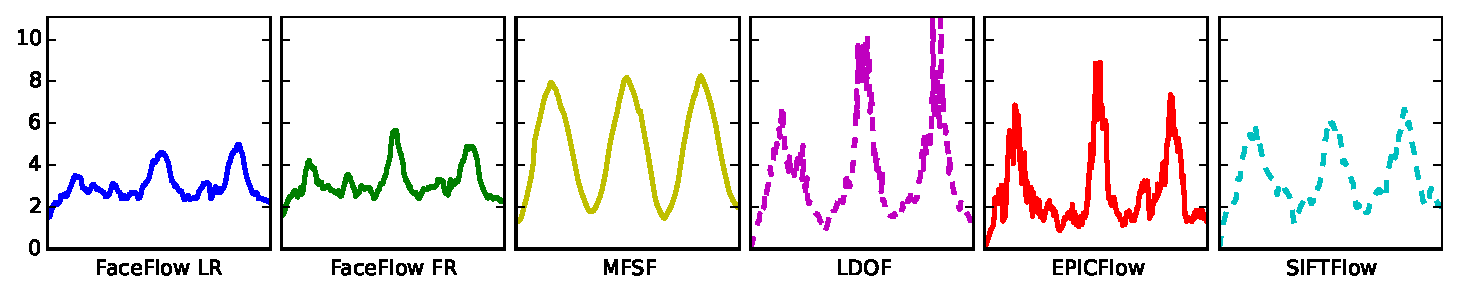
\includegraphics[width=\textwidth]{face_flow/images/synthetic/frame_error_5_flat}
    \end{subfigure}  \\
    \begin{subfigure}{6in}
        \centering
        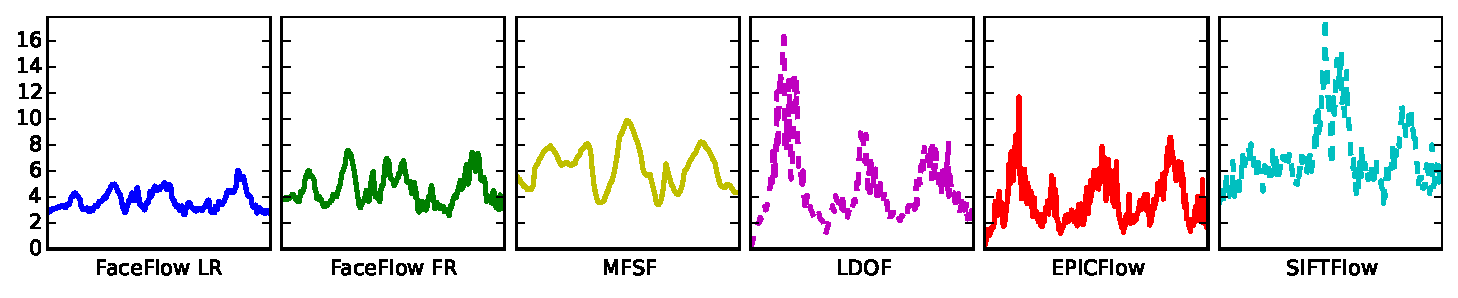
\includegraphics[width=\textwidth]{face_flow/images/synthetic/frame_error_6_flat}
    \end{subfigure}
    \caption{The average endpoint error calculated for each frame of the mocap
             sequence. Vertical axis is average endpoint error, horizontal is
             frame number. Top row is the illumination sequence, bottom row is
             illumination + occlusion.}
\label{fig:per_frame_error}
\end{figure}
%%%%%%%%%%%%%%%%%%%%%%%%%%%%%%%%%%%%%%%%%%%%%%%%%%%%%%%%%%%%%%%%%%%%%%%%%%%%%%%%
%%%%%%%%%%%%%%%%%%%%%%%%%%%%%%%%%%%%%%%%%%%%%%%%%%%%%%%%%%%%%%%%%%%%%%%%%%%%%%%%
\newcommand{\framerowreal}[1]{%
\adjustbox{valign=m,vspace=1pt}{\includegraphics[width=3.15cm,height=2.35cm]{face_flow/images/real/#1_ff_dsift_sequence}} &
\adjustbox{valign=m,vspace=1pt}{\includegraphics[width=3.15cm,height=2.35cm]{face_flow/images/real/#1_mfsf}}              &
\adjustbox{valign=m,vspace=1pt}{\includegraphics[width=3.15cm,height=2.35cm]{face_flow/images/real/#1_ldof}}              &
\adjustbox{valign=m,vspace=1pt}{\includegraphics[width=3.15cm,height=2.35cm]{face_flow/images/real/#1_epicflow}}          &
\adjustbox{valign=m,vspace=1pt}{\includegraphics[width=3.15cm,height=2.35cm]{face_flow/images/real/#1_siftflow}}
}

\setlength{\tabcolsep}{1pt}
\begin{figure}[t]
    \centering
    \begin{tabular}{cccccc}
           & Face Flow LR & MFSF & LDOF & EPICFlow & SIFTFlow \\ \vspace{-0.1cm}
        15 & \framerowreal{15}                                \\ \vspace{-0.1cm}
        21 & \framerowreal{21}                                \\ \vspace{-0.1cm}
       119 & \framerowreal{119}
    \end{tabular}
    \caption{Results on real data. Here, we incorporate the landmark constraint
             and thus do not give results for Face Flow FR.}
\label{fig:real_examples}
\end{figure}
\setlength{\tabcolsep}{6pt}
% %%%%%%%%%%%%%%%%%%%%%%%%%%%%%%%%%%%%%%%%%%%%%%%%%%%%%%%%%%%%%%%%%%%%%%%%%%%%%%%%